% !TeX root = RJwrapper.tex
\title{Converting LaTeX Legacy R Journal Articles into R Markdown Articles using texor and rebib}


\author{by Abhishek Ulayil, Mitch O'Hara-Wild, Christophe Dervieux, Heather Turner, and Dianne Cook}

\maketitle

\abstract{%
An abstract of less than 150 words.
}

\hypertarget{introduction}{%
\section{Introduction}\label{introduction}}

The R Journal is the primary open-access outlet for publications produced by the R community. It was born in 2008, evolving from a newsletter, that ran from 2001, into a more formal article publication to encourage documenting statistical computing research.

The format is constantly evolving. Early articles were typeset using LateX (The LaTeX Project 2023), from a specific, but changing, template. This requires that code is separated from the documentation, and there is a chance that code chunks in the paper don't reproduce the results reported. With the emergence of dynamic document systems like R Markdown (Xie, Allaire, and Grolemund 2018) a tight-coupling of code and documentation is possible. Code chunks are dynamically executed when the document is typeset using a system like \CRANpkg{knitr} (Xie 2015), making reporting of computing research more reproducible.

In 2019, with the help of funding from the R Consortium it was decided that it was time to update operations. One aspect of this was to change from LaTeX paper submissions to a more reproducible format, where code was embedded in the document, and the output could be both HTML and pdf. There are numerous benefits of HTML format:

\begin{enumerate}
\def\labelenumi{\arabic{enumi}.}
\tightlist
\item
  Articles can include interactive graphics and tables.
\item
  The format is more accessible to screen readers making the work more accessible to vision-impaired researchers.
\end{enumerate}

This latter point is a reason to consider converting all of the legacy articles into HTML.

A key decision for creating conversion software was to decide to directly convert LaTeX to HTML, or PDF to HTML, or LaTeX to R Markdown, and then use the current journal tools to create the HTML. The latter approach was decided to be the most versatile and useful. If an article can be converted from LaTeX to R Markdown, it would help authors make the transition to reproducible publishing, beyond what the R Journal needed. Once an article is in R Markdown format it can be adapted to include the code for dynamic execution.

In addition to article format, changes to the web site structure were important for delivering the publication. Web site architectures are also constantly evolving, and the emergence of \CRANpkg{distill} (Dervieux et al. 2022) allows for the journal web site to optimally deliver R Markdown articles.

The \CRANpkg{rjtools} was developed to create articles using R Markdown for the R Journal, and to embed them into the journal web site. The packages described here, \CRANpkg{texor} and \CRANpkg{rebib} describes software to convert legacy LaTeX format articles into Rmarkdown, so that they can be rendered in HTML in the new web site.

The paper is organised as follows. Section XXX gives an overview of the conversion process. Section XXX describes examples of pre-processing using regular expressions, and section XXX provides examples of post-processing using lua filters. Section XXX describes tools to do special handling of bibliography files. Section XXX runs through an example conversion process.

\hypertarget{the-internals-of-converting-from-latex-to-r-markdown}{%
\section{The internals of converting from LaTeX to R Markdown}\label{the-internals-of-converting-from-latex-to-r-markdown}}

The decision to convert to R Markdown format means that the final output to pdf and HTML will depend on Pandoc (MacFarlane 2023). Pandoc is a versatile document conversion program written in Haskell that is core to numerous documentation systems, including R Markdown and Quarto. Pandoc first converts a document into an abstract syntax tree. From this, it can convert to a different format, including custom ones.

Pandoc can be used to do the conversion from LaTeX to R Markdown also. However, additional pre-processing needs to be done to handle special R Journal LaTeX styling. And further post-processing needs to be done to handle specific R Journal R Markdown styling. The \CRANpkg{texor} package contains functionality to handle this pre- and postprocessing of the document.

\textbf{DC: Add a diagram here showing flow of work, just pre-process .tex -\textgreater{} pandoc -\textgreater{} lua ; rebib operations???}

The supplementary materials has example folders containing LaTeX documents that allow the reader to see how different common patterns in the legacy documents are handled with the conversion. These include:

\begin{itemize}
\tightlist
\item
  \texttt{code-env}: Explains how different code environments defined by the R Journal style are handled, and additional details such as code in figure environments, and code in table environments.
\item
  \texttt{math-env}: Examples of inline math, display math, how equation numbering is handled by a Lua filter to convert from LaTeX labelling to R Markdown labelling.
\item
  \texttt{figure-env}: Explains how the variety of figure definitions are handled in the conversion, including different image formats, numbering, captions, labelling, multiple images, and \texttt{tikz} (Josh Cassidy 2013) images.
\item
  \texttt{table-env}: Examples of how a variety of table types are converted, including multicolumn, complex and wide tables.
\item
  \texttt{lua-filters}: Overview and lots of small examples of Lua filters to handle the custom output needed for the R Markdown format.
\item
  \texttt{metadata}: This has a collection of additional format handling including extracting metadata like author names and affiliations, article identifiers used in the review process, and handling citations, footnotes and links.
\item
  \texttt{bibliography}: The bibliography was handled differently over the years of the journal, and this details how to use the \texttt{rebib} functionality to handle \texttt{bbl} files, embedded \texttt{bbl}, to convert into the standard \texttt{.bib} format.
\end{itemize}

The explanations in the next sections are extracted from these examples. In each of these folders there is a \texttt{RJwrapper.tex}, and \texttt{.tex} file, with the extra template files \texttt{RJournal.sty} and \texttt{Rlogo-5.png}. These match the legacy template file structure, from which the \texttt{RJwrapper.pdf} file is created. If you follow the instructions in the \texttt{README.md} you can create the R Markdown and HTML versions of the document.

\hypertarget{pre-processing-using-regular-expressions}{%
\subsection{Pre-processing using regular expressions}\label{pre-processing-using-regular-expressions}}

LaTeX is very descriptive language, that allows authors substantial freedom for customization. Markdown (Gruber 2002), on which R Markdown is based, is more restrictive and was born to make it easier to create web pages without the distraction of a gazillion HTML tags. The beauty of Markdown is that it allows the author to focus on writing, without format cluttering the text. The drawback is that it is simple typesetting, optimized for web delivery.

While pandoc can do most of the heavy-lifting, it cannot cope with all the freedom with which LaTeX documents are written. An example of this is with formatting of code. Pandoc only handles the \texttt{verbatim} environment, but there are many ways to format code in LaTeX, and the R Journal template has a special \texttt{\textbackslash{}code\{\}} command. If the code environment is not verbatim, then pandoc will also try to process the actual code content as LaTeX commands and will likely lose details. It is better to convert these synonyms into \texttt{verbatim} environments this prior to passing the document to pandoc.

The functions in \CRANpkg{texor} that handle the pre-processing using regular expressions are:

\begin{itemize}
\tightlist
\item
  \texttt{stream\_editor()}: operates like the \texttt{sed} function in unix (Ritchie and Thompson 1978) and allows generic text pattern matching and replacing.
\item
  \texttt{patch\_code\_env()}: replaces the common code environments, \texttt{code}, \texttt{example}, \texttt{Sin}, \texttt{Sout}, \texttt{Scode}, \texttt{Sinput}, \texttt{smallverbatim}, \texttt{boxedverbatim}, \texttt{smallexample} with \texttt{verbatim}.
\item
  \texttt{patch\_equations()}: coordinates various equation environments.
\item
  \texttt{patch\_figure\_env()}: coordinates various figure environments.
\item
  \texttt{patch\_table\_env()}: coordinates table environments.
\end{itemize}

These functions are verbose and describe all the changes being made. They also create a backup of the original file before making the changes.

\hypertarget{post-processing-using-lua-filters}{%
\subsection{Post-processing using Lua filters}\label{post-processing-using-lua-filters}}

Lua (Ierusalimschy, Figueiredo, and Filho 1996) is a programming language, that is light-weight, fast, ideal for procedural operations. It is embedded in many other applications to allow custom scripting for extensibility. Pandoc allows users to provide custom lua filters to produce custom output formats. The \CRANpkg{texor} package handles post-processing of the R Markdown document into the special format for the R Journal using a suite of Lua filters.

Here is an example of a Lua filter available in \CRANpkg{texor}:

\begin{verbatim}
function Div(el)
    if el.classes[1] == 'thebibliography' then
        return { }
    end
end
\end{verbatim}

This filter reads the abstract syntax tree, selecting all the Div elements. Then it looks for the class ``thebibliography.'' This Div element contains the LaTeX bibliographic records, that appear at the very end of papers. It should not be in the document when using the ``RJ-web-article'' layout, because it is added from meta-data when the R Markdown is knitted. So the Lua filter removes this section.

\hypertarget{handling-figures}{%
\subsection{Handling figures}\label{handling-figures}}

Figure definitions in LaTeX are many and varied! The standard, single figure definition with the \texttt{figure} environment is handled by pandoc, which converts:

\begin{verbatim}
\begin{figure}[htbp]
  \centering
  
\includegraphics[width=0.35\textwidth]{Rlogo-5.png}
  \caption{The logo of R.}
  \label{figure:rlogo}
\end{figure}
\end{verbatim}

to

\begin{verbatim}
<figure id="figure:rlogo">
<img src="Rlogo-5.png" style="width:35.0%" />
<figcaption>Figure 1: The logo of R.</figcaption>
</figure>
\end{verbatim}

PDF figures cause a problem for HTML display, so the image is first converted to PNG, in the pre-processing of the LaTeX document. Then the figure environment would be post-processed using pandoc, as described above.

Multiple figures are supported with the latest versions of pandoc, so definitions like:

\begin{verbatim}
\begin{figure*}[htbp]
  \centering
  
\includegraphics[width=0.45\textwidth]{Rlogo-5.png}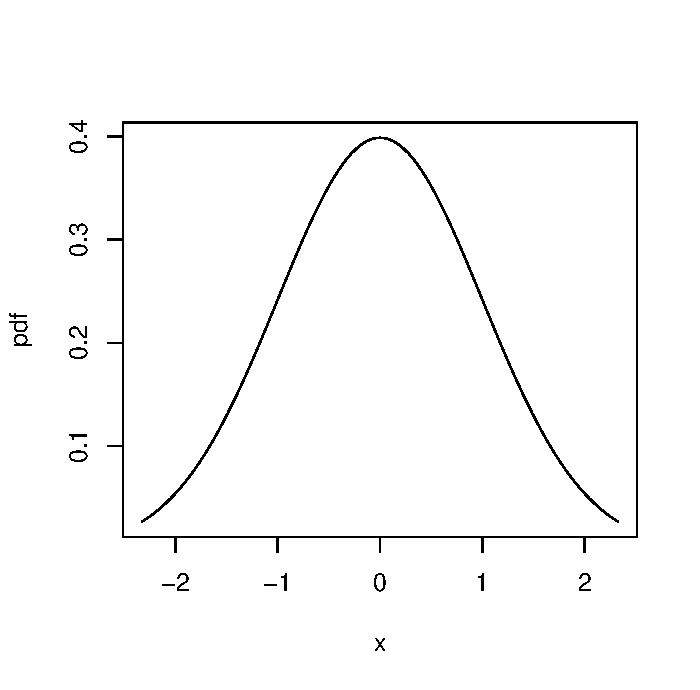
\includegraphics[width=0.45\textwidth]{normal}
  \caption{Images side by side}
  \label{fig:twoimages}
\end{figure*}
\end{verbatim}

will be converted to:

\begin{verbatim}
<figure id="fig:twoimages">
<p><img src="Rlogo-5.png" style="width:45.0%" alt="image" /><img
src="normal.png" style="width:45.0%" alt="image" /></p>
<figcaption>Figure 3: Images side by side</figcaption>
</figure>
\end{verbatim}

Some legacy articles defined images using \texttt{tikz} commands, such as:

\begin{verbatim}
\begin{figure}

%% Generated Image will included as a PNG above automatically
  \centering
\tikzstyle{process} = [rectangle, rounded corners,
minimum width=3cm, 
minimum height=1cm,
text centered, 
draw=black]
\tikzstyle{arrow} = [thick,->,>=stealth]
\begin{tikzpicture}[node distance=4cm]
%Nodes
...
\end{verbatim}

This is handled by pre-rpocessing the LaTeX to create the image, as both PDF, and them PNG, for inclusion in the R Markdown document using:

\begin{verbatim}
<figure id="fig:tikz">
<img src="tikz/figtikz.png" style="width:100.0%" />

<figcaption>Figure 5: Tikz Image example</figcaption>
</figure>
\end{verbatim}

Interestingly, some legacy articles have algorithms are defined in the figure environment:

\begin{verbatim}
\begin{algorithm}[htbp]
\SetAlgoLined
\KwData{this text}
\KwResult{how to write algorithm with \LaTeX2e }
initialization\;
\While{not at end of this document}{
read current\;
\eIf{understand}{
go to next section\;
current section becomes this one\;
}{
go back to the beginning of current section\;
}
}
\caption{How to write algorithms}
  \label{alg:how}
\end{algorithm}
\end{verbatim}

\hypertarget{handling-equations}{%
\subsection{Handling equations}\label{handling-equations}}

\hypertarget{handling-the-bibliography}{%
\subsection{Handling the bibliography}\label{handling-the-bibliography}}

\hypertarget{logging-the-conversion}{%
\subsection{Logging the conversion}\label{logging-the-conversion}}

\hypertarget{one-step-user-facing-conversion}{%
\subsection{One-step user-facing conversion}\label{one-step-user-facing-conversion}}

The only function that a user necessarily needs is \texttt{latex\_to\_web()}. This creates the R Journal style R Markdown file from a given R Journal style LaTeX file.
This is achieved in several conversion steps, \texttt{convert\_to\_markdown()}, \texttt{generate\_rmd()} and \texttt{produce\_html()}.

\hypertarget{using}{%
\section{\texorpdfstring{Using \CRANpkg{texor}}{Using }}\label{using}}

The package \texttt{texor} can be installed from CRAN using:

\begin{verbatim}
install.packages("texor")
\end{verbatim}

and the development version from \url{https://abhi-1u.github.io/texor}.

\textbf{Examples / getting started / usage and so on}

Run through the different examples in supplementary here

\textbf{From general LaTeX to generic R Markdown}

\hypertarget{managing-the-bibliography-using}{%
\section{\texorpdfstring{Managing the bibliography using \CRANpkg{rebib}}{Managing the bibliography using }}\label{managing-the-bibliography-using}}

\hypertarget{overview}{%
\subsection{Overview}\label{overview}}

The \CRANpkg{rebib} package addresses the issue with LaTeX articles using built-in bibliography options with or without BibTeX files. While this works well with LaTeX, it won't work with Rmarkdown. Initially the goal was to use external software like Biber to convert the embedded bibliography to BibTeX.
However the integration of external software was not viable, hence the experimental idea of a bibliography parser gained momentum.

It was initially a part of the \CRANpkg{texor} package, as those functions grew in features and became more involved; at that point, it made sense to move those functions as a separate package. Initially, there were some reservations about
the usage of \CRANpkg{rebib} and its stability with various formats. However, the package has improved over time and proven to be a good performer.

\hypertarget{using-1}{%
\subsection{\texorpdfstring{Using \CRANpkg{rebib}}{Using }}\label{using-1}}

\textbf{Install instructions}

\textbf{Examples / getting started / usage and so on}

\hypertarget{summary}{%
\section{Summary}\label{summary}}

Only handling to html format, especially relevant for figures, because the legacy pdf will remain the same. If using for converting work from LaTeX to Rmd then this will need manual changing by author. See rjtools guide.

Where this might be useful in the future, other applications.

No shift to quarto yet.

Known problems that need manual fixes.

\hypertarget{acknowledgments}{%
\section{Acknowledgments}\label{acknowledgments}}

pandoc
``TODO : Later''

\hypertarget{supplementary-materials}{%
\section{Supplementary materials}\label{supplementary-materials}}

Several supplementary example documents are provided which illustrate how different elements of LaTeX-authored papers are handled. These are:

\begin{itemize}
\tightlist
\item
\end{itemize}

The GitHub repos supporting this work are:

\begin{itemize}
\tightlist
\item
  \CRANpkg{texor}: \url{https://abhi-1u.github.io/texor}
\item
  \CRANpkg{rebib}: \url{https://abhi-1u.github.io/rebib/}
\item
  This paper: \url{https://github.com/Abhi-1U/texor-rjarticle}
\item
  More details on \CRANpkg{rjtools} are at \url{https://rjournal.github.io/rjtools/}
\end{itemize}

\hypertarget{references}{%
\section*{References}\label{references}}
\addcontentsline{toc}{section}{References}

\hypertarget{refs}{}
\begin{CSLReferences}{1}{0}
\leavevmode\vadjust pre{\hypertarget{ref-distill}{}}%
Dervieux, Christophe, JJ Allaire, Rich Iannone, Alison Presmanes Hill, and Yihui Xie. 2022. \emph{Distill: 'R Markdown' Format for Scientific and Technical Writing}. \url{https://CRAN.R-project.org/package=distill}.

\leavevmode\vadjust pre{\hypertarget{ref-markdown}{}}%
Gruber, John. 2002. {``Markdown.''} https://daringfireball.net/projects/markdown/.

\leavevmode\vadjust pre{\hypertarget{ref-lua}{}}%
Ierusalimschy, Roberto, Luiz Henrique de Figueiredo, and Waldemar Celes Filho. 1996. {``Lua---an Extensible Extension Language.''} \emph{Software: Practice and Experience} 26 (6): 635--52.

\leavevmode\vadjust pre{\hypertarget{ref-casflow}{}}%
Josh Cassidy. 2013. \emph{{LaTeX Graphics using TikZ: A Tutorial for Beginners (Part 3)---Creating Flowcharts}}. Overleaf tutorials. \url{https://www.overleaf.com/learn/latex/}.

\leavevmode\vadjust pre{\hypertarget{ref-pandoc}{}}%
MacFarlane, John. 2023. {``Pandoc: A Universal Document Converter.''} https://pandoc.org.

\leavevmode\vadjust pre{\hypertarget{ref-unix}{}}%
Ritchie, O. M., and K. Thompson. 1978. {``The UNIX Time-Sharing System.''} \emph{The Bell System Technical Journal} 57 (6): 1905--29. \url{https://doi.org/10.1002/j.1538-7305.1978.tb02136.x}.

\leavevmode\vadjust pre{\hypertarget{ref-latex}{}}%
The LaTeX Project. 2023. {``LaTeX -- a Document Preparation System.''} https://www.latex-project.org.

\leavevmode\vadjust pre{\hypertarget{ref-knitr}{}}%
Xie, Yihui. 2015. \emph{Dynamic Documents with {R} and Knitr}. 2nd ed. Boca Raton, Florida: Chapman; Hall/CRC. \url{https://yihui.org/knitr/}.

\leavevmode\vadjust pre{\hypertarget{ref-rmarkdown}{}}%
Xie, Yihui, J. J. Allaire, and Garrett Grolemund. 2018. \emph{R Markdown: The Definitive Guide}. Boca Raton, Florida: Chapman; Hall/CRC. \url{https://bookdown.org/yihui/rmarkdown}.

\end{CSLReferences}

\bibliography{RJreferences.bib}

\address{%
Abhishek Ulayil\\
Institute of Actuaries of India (student)\\%
Mumbai, India\\
%
%
\textit{ORCiD: \href{https://orcid.org/0009-0000-6935-8690}{0009-0000-6935-8690}}\\%
\href{mailto:perricoq@outlook.com}{\nolinkurl{perricoq@outlook.com}}%
}

\address{%
Mitch O'Hara-Wild\\
Monash University\\%
Melbourne, Australia\\
%
%
\textit{ORCiD: \href{https://orcid.org/0000-0001-6729-7695}{0000-0001-6729-7695}}\\%
\href{mailto:mail@mitchelloharawild.com}{\nolinkurl{mail@mitchelloharawild.com}}%
}

\address{%
Christophe Dervieux\\
Posit PBC\\%
Paris, France\\
%
%
\textit{ORCiD: \href{https://orcid.org/0000-0003-4474-2498}{0000-0003-4474-2498}}\\%
\href{mailto:christophe.dervieux@gmail.com}{\nolinkurl{christophe.dervieux@gmail.com}}%
}

\address{%
Heather Turner\\
University of Warwick\\%
Newport, United Kingdom\\
%
%
\textit{ORCiD: \href{https://orcid.org/0000-0002-1256-3375}{0000-0002-1256-3375}}\\%
\href{mailto:ht@heatherturner.net}{\nolinkurl{ht@heatherturner.net}}%
}

\address{%
Dianne Cook\\
Monash University\\%
Melbourne, Australia\\
%
%
\textit{ORCiD: \href{https://orcid.org/0000-0002-3813-7155}{0000-0002-3813-7155}}\\%
\href{mailto:dicook@monash.edu}{\nolinkurl{dicook@monash.edu}}%
}
